\documentclass[notheorems,mathserif,table,compress]{beamer}  %dvipdfm选项是关键,否则编译统统通不过
%%------------------------常用宏包------------------------
%%注意, beamer 会默认使用下列宏包: amsthm, graphicx, hyperref, color, xcolor, 等等
\usepackage{fontspec,xunicode,xltxtra}
\usepackage{amsfonts,amssymb}  % for XeTeX
%%------------------------ThemeColorFont------------------------
%% Presentation Themes
% \usetheme[<options>]{<name list>}
\usetheme{Madrid}
%% Inner Themes
% \useinnertheme[<options>]{<name>}
%% Outer Themes
% \useoutertheme[<options>]{<name>}
\useoutertheme{miniframes} 
%% Color Themes 
% \usecolortheme[<options>]{<name list>}
%% Font Themes
% \usefonttheme[<options>]{<name>}
\setbeamertemplate{background canvas}[vertical shading][bottom=white,top=structure.fg!7] %%背景色, 上25%的蓝, 过渡到下白.
\setbeamertemplate{theorems}[numbered]
\setbeamertemplate{navigation symbols}{}   %% 去掉页面下方默认的导航条.
\usepackage{zhfontcfg}
\usepackage{iplouclistings}
\usepackage{fancybox}
\usepackage{latexsym}
\usepackage{xcolor}
\usepackage{subfigure} %%图形或表格并排排列
\newcommand\zhyfly[2][purple]{\hskip5pt\shadowbox{\color{#1}\small\lishu #2\vspace{2mm}}}
%\setsansfont[Mapping=tex-text]{文泉驿正黑}  %% 需要fontspec宏包
     %如果装了Adobe Acrobat,可在font.conf中配置Adobe字体的路径以使用其中文字体
     %也可直接使用系统中的中文字体如SimSun,SimHei,微软雅黑 等
     %原来beamer用的字体是sans family;注意Mapping的大小写,不能写错
     %设置字体时也可以直接用字体名,以下三种方式等同:
     %\setromanfont[BoldFont={黑体}]{宋体}
     %\setromanfont[BoldFont={SimHei}]{SimSun}
     %\setromanfont[BoldFont={"[simhei.ttf]"}]{"[simsun.ttc]"}
%%------------------------MISC------------------------
\graphicspath{{figures/}}         %% 图片路径. 本文的图片都放在这个文件夹里了.
%%------------------------正文------------------------
\begin{document}
\XeTeXlinebreaklocale "zh"         % 表示用中文的断行
\XeTeXlinebreakskip = 0pt plus 1pt % 多一点调整的空间
%%----------------------------------------------------------
%% This is only inserted into the PDF information catalog. Can be left
%% out.
%%%
%% Delete this, if you do not want the table of contents to pop up at
%% the beginning of each subsection:
\AtBeginSection[]{                              % 在每个Section前都会加入的Frame
  \frame<handout:0>{
    \frametitle{内容提要}\small
    \tableofcontents[current,currentsubsection]
  }
}
\AtBeginSubsection[]                            % 在每个子段落之前
{
  \frame<handout:0>                             % handout:0 表示只在手稿中出现
  {
    \frametitle{下一节内容}\small
    \tableofcontents[current,currentsubsection] % 显示在目录中加亮的当前章节
  }
}
%%----------------------------------------------------------
\title[图像频域显著性检测]{图像频域显著性检测}
%\subtitle{Mathematics of Scientific Computing}
\author[赵红苗]{姓~~名~~~~~\textcolor{olive}{赵红苗}\\
    导~~师~~~~~\textcolor{olive}{郑海永}}
\institute[中国海洋大学]{\kaishu\small\textcolor{violet}{中国海洋大学~~信息科学与工程学院}}
\date{2015~年~5~月~23~日}
\titlegraphic{

\includegraphics[height=2cm]{ouc-logo.png}}
%\titlegraphic{\vspace{-6em}\includegraphics[height=7cm]{ouc}\vspace{-6em}}
\frame{ \titlepage }
%%----------------------------------------------------------
\section*{目录}
\frame{\frametitle{目录}\tableofcontents}
%%============================================================================================================================
\section{课题背景}
%\subsection{选题背景及意义}%如果你想书签不出现问题,请不要用\XeTeX
 
%-----------------------------------------------------------------------------------------------------------------------------
%\begin{frame}
%  \frametitle{视觉注意}
%\begin{figure}[!htb] %插图
%\centering
%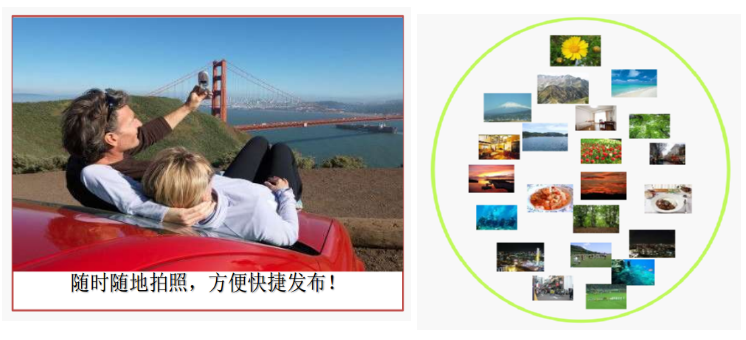
\includegraphics[width=0.9\textwidth]{network1.png}
%\caption{互联网用户上传数千亿幅照片}
%\label{fig:1}
%\end{figure}
  % \XeTeXpicfile "./logo.jpg" xscaled 100 yscaled 100 %插图也没有问题
%\end{frame}

%-----------------------------------------------------------------------------------------------------------------------------
\begin{frame}
  \frametitle{选题背景及意义}
  \begin{itemize}
  \item 视觉注意
  \end{itemize}
\begin{figure}[!htb] %插图
\centering
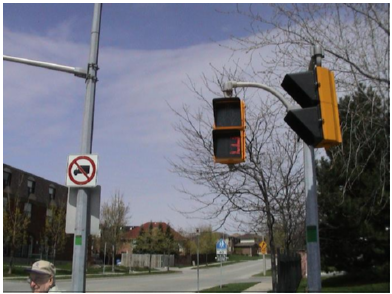
\includegraphics[width=0.7\textwidth]{nature.png}
%\caption{互联网用户上传数千亿幅照片}
\label{fig:2}
\end{figure}
  % \XeTeXpicfile "./logo.jpg" xscaled 100 yscaled 100 %插图也没有问题
\end{frame}

%-----------------------------------------------------------------------------------------------------------------------------
\begin{frame}
  \frametitle{选题背景及意义}
\begin{figure}[!htb] %插图
\centering
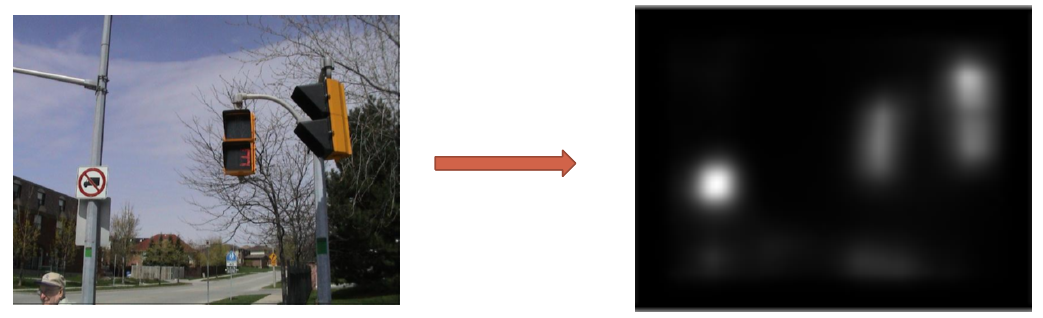
\includegraphics[width=0.95\textwidth]{视觉注意1.png}
%\caption{互联网用户上传数千亿幅照片}
\label{fig:2}
\end{figure}
  \begin{itemize}
  \item 目标检测、图像分割、以及图像和视频压缩等
  \end{itemize}
  % \XeTeXpicfile "./logo.jpg" xscaled 100 yscaled 100 %插图也没有问题
\end{frame}
%-----------------------------------------------------------------------------------------------------------------------------
%\begin{frame}
%  \frametitle{视觉注意}
%  \begin{enumerate}
%  \item 定义 
%  \begin{itemize}
%  \item 人类视觉系统在面对复杂场景时,会迅速将注意力集中在少数重要区域,并利用有限的处理能力对其优先处理。
%  \end{itemize}
%  \item 意义
%  \begin{itemize}
%  \item 视觉注意机制可以忽略图像中的冗余信息以及无关信息,从而提高图像处理的效率;
%  \item 利用视觉注意机制可以使得图像处理结果更加符合使用者的直观感受。
%  \end{itemize}
%  \end{enumerate}
%\end{frame}

%-----------------------------------------------------------------------------------------------------------------------------
%\begin{frame}
%  \frametitle{显著性检测}
%  \begin{enumerate}
%  \item 给定一幅图像,判断图像中哪些区域对于人眼来说是显著的,并用灰度进行量化。
%  \item 显著图

%\begin{figure}[!htb] %插图
%\centering
%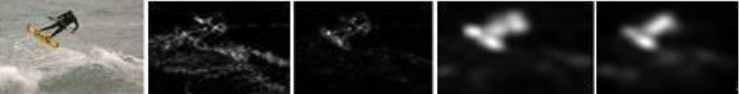
\includegraphics[width=0.75\textwidth]{各种显著图.png}
%\caption{互联网用户上传数千亿幅照片}
%\label{fig:3}
%\end{figure}

%  \item 应用
%  \begin{itemize}
%  \item 目标检测,图像分割,以及图像和视频压缩等。
%  \end{itemize}
%  \end{enumerate}
%\end{frame}

%-----------------------------------------------------------------------------------------------------------------------------
\begin{frame}
  \frametitle{选题背景及意义}

  \begin{itemize}
  \item 空间域模型\textcolor{red}{计算量较大,比较耗时}
  \item 基于信息论和统计模型需要\textcolor{red}{引入大量参数}
  \item \color{blue} \fbox{频域处理简单、高效及参数设置少}
  \end{itemize}
\end{frame}

%-----------------------------------------------------------------------------------------------------------------------------
\begin{frame}
  \frametitle{课题来源}
  \begin{enumerate}%[<+-| structure@+>]
  \item \rowcolors[]{1}{blue!18}{blue!7}
  \begin{tabular}[c]{c|p{6.6cm}}
    %\hline
    项目类别 & 国家自然科学基金\\
    %\hline
    课题名称 & {\heiti 基于视觉注意结合生物形态特征的海洋}\\
              & {\heiti 浮游植物显微图像分析}\\
    %\hline
    课题编号 & 61301240\\
    %\hline
    起止年限 & 2014.01~$\sim$~2016.12\\
    %\hline
  \end{tabular}
  \vspace{5mm}
  \item \rowcolors[]{1}{blue!18}{blue!7}
  \begin{tabular}[c]{c|p{6.6cm}}
    %\hline
    项目类别 & 国家自然科学基金\\
    %\hline
    课题名称 & {\heiti 基于生物形态特征的中国海常见有害赤}\\
              & {\heiti 潮藻显微图像识别}\\
    %\hline
    课题编号 & 61271406\\
    %\hline
    起止年限 & 2013.01~$\sim$~2016.12\\
    %\hline
  \end{tabular}
  \end{enumerate}
\end{frame}

%-----------------------------------------------------------------------------------------------------------------------------
%\begin{frame}
%  \frametitle{选题背景}
%\begin{center}
%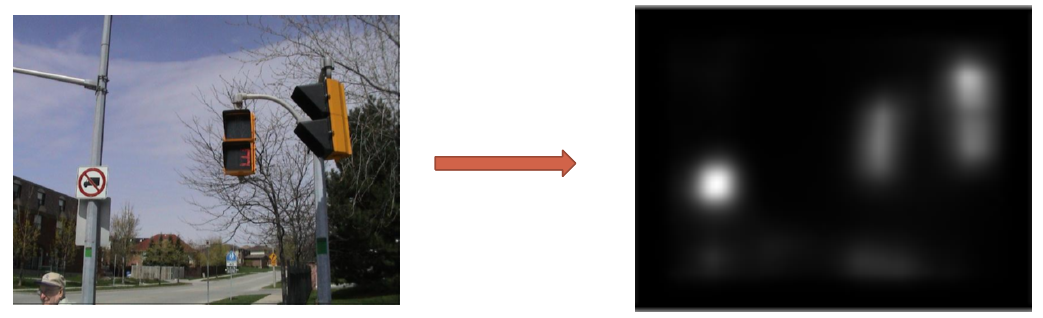
\includegraphics[width=0.80\linewidth]{视觉注意1.png} \\%
%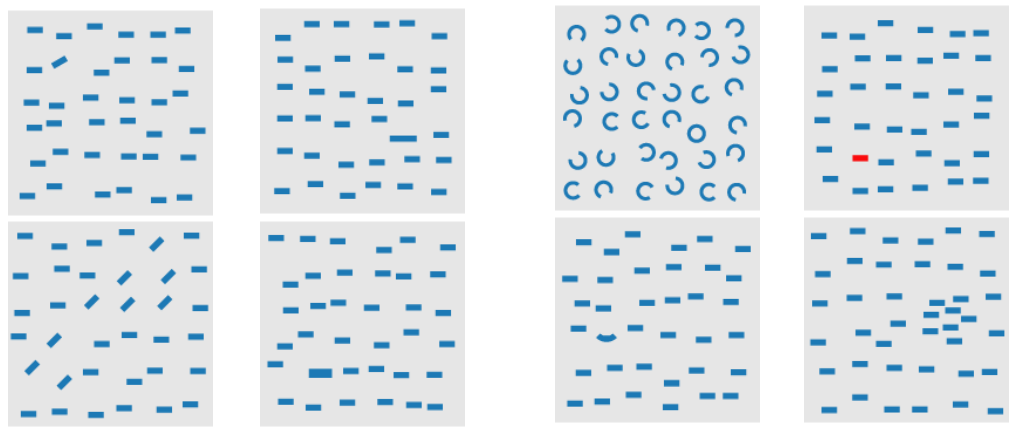
\includegraphics[width=0.80\linewidth]{视觉注意2.png}%
%\end{center}
%\pause
%\end{frame}

%-----------------------------------------------------------------------------------------------------------------------------
%\begin{frame}
%  \frametitle{选题背景}
%\begin{center}
%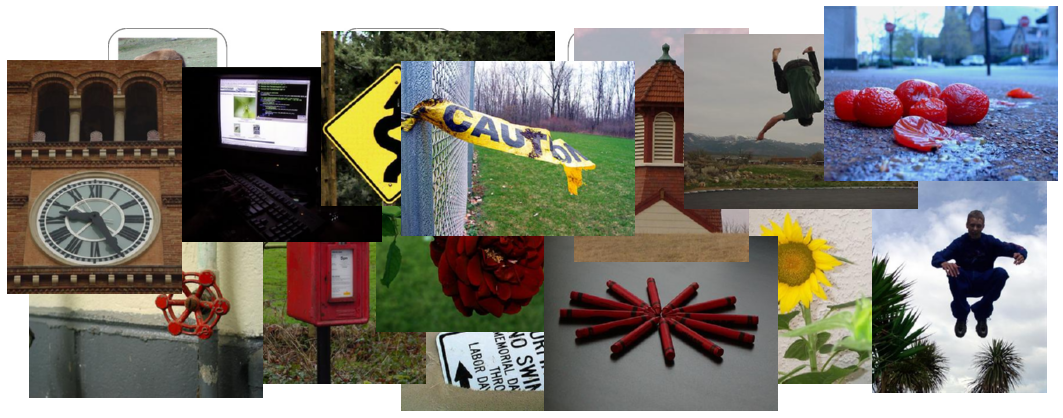
\includegraphics[width=0.80\linewidth]{绪论多幅图片.png}%
%\end{center}
%\pause
%\begin{itemize}
%\item 视觉注意机制提高了视觉系统的信息处理效率;
%\item 视觉注意计算模型越来越多的应用到计算机视觉领域;
%\item 空间域视觉注意模型计算量相对较大,比较耗时,而频域处理具有简单、高效及参数设置少的特点。
%\end{itemize}
%\end{frame}

%-----------------------------------------------------------------------------------------------------------------------------
%\begin{frame}
%  \frametitle{选题背景}
%\begin{center}
%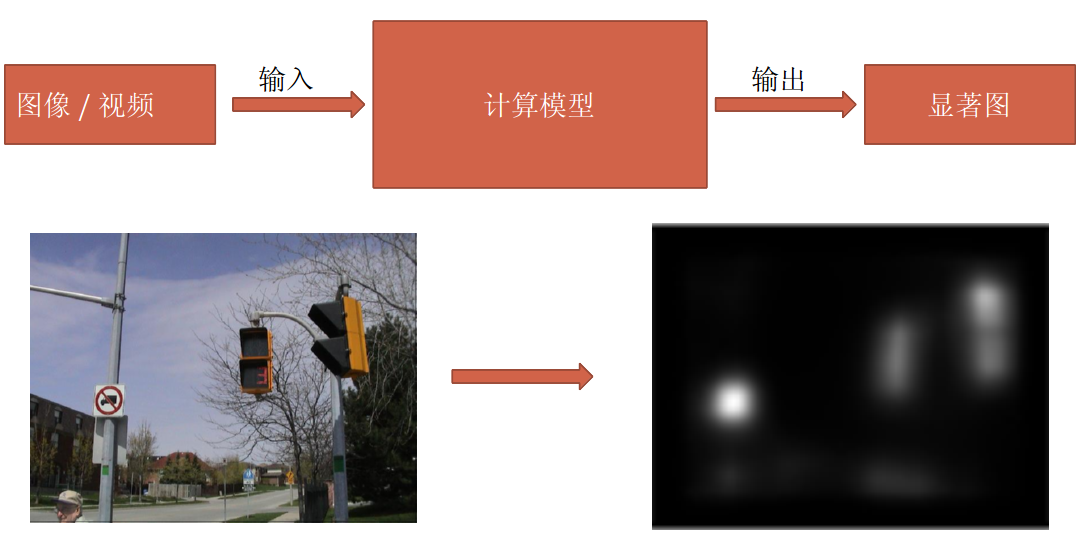
\includegraphics[width=0.88\linewidth]{视觉注意.png}%
%\end{center}
%\pause
%\end{frame}

%=============================================================================================================================
\section{频域显著性检测}
%\subsection{4.6.1 Basic Concepts}%如果你想书签不出现问题,请不要用\XeTeX
                                 %这类复杂的指令,直接写XeTeX吧
\begin{frame}
  \frametitle{频域显著性检测一般步骤}
\begin{center}
\includegraphics[width=0.85\linewidth]{图2_1.jpg}%
\end{center}
  \begin{itemize}
  \item 预处理$\Longrightarrow$提取图像显著性特征
  \item 后处理$\Longrightarrow$增强图像的显著对比度
  \item 频域处理$\Longrightarrow$\textcolor{blue}{幅度谱}(相位谱保持不变)
  \end{itemize}

\end{frame}


%-----------------------------------------------------------------------------------------------------------------------------
%\begin{frame}
%  \frametitle{预处理}
%\begin{itemize}
%\item RGB彩色模型;
%\item Lab 彩色模型;
%\item IRGBY 彩色模型;
%\item 图像尺度调整模型;
%\end{itemize}
%\pause
%\end{frame}

%-----------------------------------------------------------------------------------------------------------------------------
%\begin{frame}
%  \frametitle{时频变换}
%\begin{itemize}
%\item 傅里叶变换;
%\item 离散余弦变换;
%\item 小波变换;
%\item 四元数傅里叶变换;
%\end{itemize}
%\pause
%\end{frame}

%=============================================================================================================================
%\section{频域显著性检测模型}
%-----------------------------------------------------------------------------------------------------------------------------
\begin{frame}
  \frametitle{幅度谱处理 }
  \begin{enumerate}
  \item \textrm{SR}模型 
  \begin{itemize}
  \item 保留图像的\textcolor{blue}{剩余谱}:$\mathcal{R}(f)=\mathcal{L}(f)-\mathcal{A}(f)$
  \item 不足:仅突出\textcolor{red}{轮廓}或\textcolor{red}{纹理密集}的区域
  \end{itemize}
\pause
  \item \textrm{PQFT}模型
  \begin{itemize}
  \item 只保留图像的\textcolor{blue}{相位谱}信息
  \item 不足:仅突出\textcolor{red}{轮廓}或\textcolor{red}{纹理密集}的区域
  \end{itemize}
\pause
  \item \textrm{HFT}模型
  \begin{itemize}
  \item 对\textcolor{blue}{幅度谱}进行多尺度滤波
  \item 不足:显著目标检测\textcolor{red}{不正确}或\textcolor{red}{不均匀}
  \end{itemize}
  \end{enumerate}
%\pause
\end{frame}

%-----------------------------------------------------------------------------------------------------------------------------
%\begin{frame}
%  \frametitle{相位谱四元傅里叶变换显著性检测模型(PQFT)}
%  \begin{enumerate}
%  \item 核心思想
%  \begin{itemize}
%  \item 图像的相位谱即图像中的显著区域
%  \end{itemize}
%  \item 处理
%  \begin{itemize}
%  \item 只保留图像的相位谱信息
%  \end{itemize}
%  \item 评价
%  \begin{itemize}
%  \item 优点:该算法比SR算法更简单;
%  \item 缺点:没有利用图像的幅度谱信息,只能检测显著目标的边缘,无法突出整个显著目标。
%  \end{itemize}
%  \end{enumerate}
%\end{frame}

%-----------------------------------------------------------------------------------------------------------------------------
%\begin{frame}
%  \frametitle{基于频域尺度空间分析的显著性检测模型 (HFT)}
%  \begin{enumerate}
%  \item 核心思想
%  \begin{itemize}
%  \item 提出了谱尺度空间
%  \end{itemize}
%  \item 处理
%  \begin{itemize}
%  \item 对幅度谱进行多尺度滤波;
%  \item 图像熵
%  \end{itemize}
%  \item 评价
 % \begin{itemize}
%  \item 优点:可以突出整个显著目标;
%  \item 缺点:显著目标检测不正确或不均匀。
%  \end{itemize}
%  \end{enumerate}
%\end{frame}

%=============================================================================================================================
\section{基于幅度谱分析的显著目标检测模型}
%-----------------------------------------------------------------------------------------------------------------------------
\subsection{幅度谱分析}

\begin{frame}
  \frametitle{图像的重复模式}

\begin{center}
\includegraphics[width=0.42\linewidth]{new图4_2_a.png}%
\hspace{2em}
\includegraphics[width=0.36\linewidth]{new图4_2_b.png}%
\end{center}
\centering{\color{blue} \fbox{\kaishu抑制重复模式、突出显著区域}}
\end{frame}

%-----------------------------------------------------------------------------------------------------------------------------
\begin{frame}
  \frametitle{图像的重复模式}
\begin{center}
\includegraphics[width=0.82\linewidth]{图4_3.png}%
\end{center}
\centering{\color{blue} \kaishu重复模式\textcolor{magenta}{越多}$\Longrightarrow$对数幅度谱中尖刺\textcolor{magenta}{越高越尖}}
\end{frame}

%-----------------------------------------------------------------------------------------------------------------------------
\begin{frame}
  \frametitle{图像的重复模式}
\begin{center}
\includegraphics[width=0.7\linewidth]{图4_4.png}%
\end{center}
\centering{\color{blue} \kaishu重复模式\textcolor{magenta}{越多}$\Longrightarrow$对数幅度谱中尖刺\textcolor{magenta}{越高越尖}}
\end{frame}

%-----------------------------------------------------------------------------------------------------------------------------
\begin{frame}
  \frametitle{非显著性抑制分析}
\begin{center}
\includegraphics[width=0.97\linewidth]{图4_5.png}%
\end{center}
\end{frame}

%-----------------------------------------------------------------------------------------------------------------------------
%\begin{frame}
%  \frametitle{最优尺度选择分析}
%\begin{center}
%\includegraphics[width=0.85\linewidth]{图4_6.png}%
%\end{center}
%\end{frame}

%-----------------------------------------------------------------------------------------------------------------------------
%\begin{frame}
%  \frametitle{最优尺度选择分析}
%\begin{center}
%\includegraphics[width=0.7\linewidth]{图4_9.png}%
%\end{center}
%\end{frame}

%-----------------------------------------------------------------------------------------------------------------------------
\begin{frame}
  \frametitle{最优尺度选择分析}
\begin{center}
\includegraphics[width=0.4\linewidth]{图4_10.eps}%
\end{center}
\centering{\color{blue} \fbox{一维:$\sigma=\alpha\cdot(l/L)^{(-1)}$}}

\centering{\color{blue} \fbox{二维:$\sigma= \alpha\cdot\Big(\frac{f(h,w)}{f(H,W)}\Big)^{-1}$}}
\end{frame}

%------------------------------------------------------------------------------------------------------------------------------
\subsection{基于幅度谱分析频域显著目标检测算法}

%\begin{frame}
%  \frametitle{基于幅度谱分析的显著目标检测思路}

%\begin{center}
%\includegraphics[width=0.7\linewidth]{图4_12.png}%
%\end{center}
%\end{frame}

%------------------------------------------------------------------------------------------------------------------------------
\begin{frame}
  \frametitle{基于幅度谱分析的显著目标检测框架}
\begin{center}
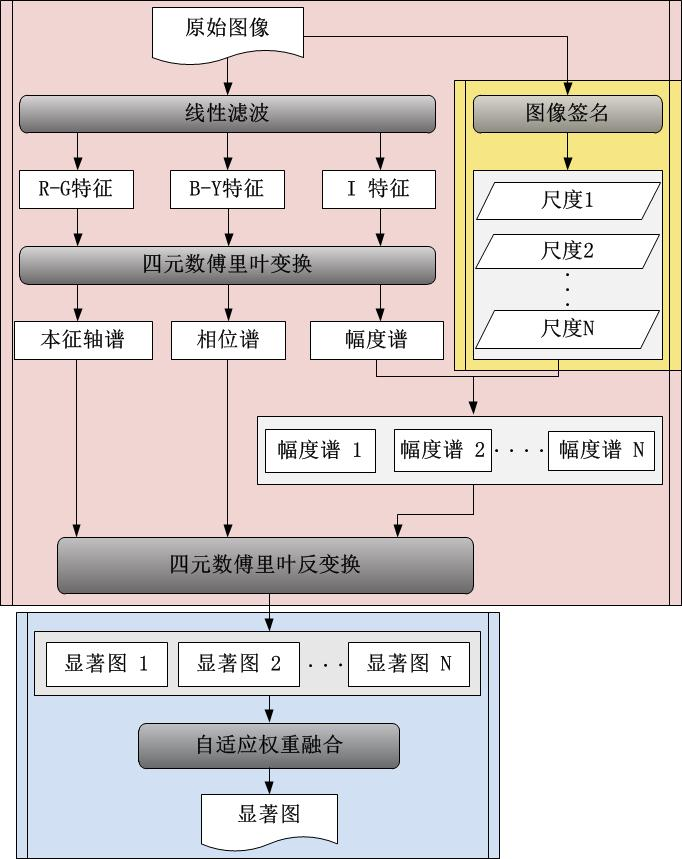
\includegraphics[width=0.42\linewidth]{frame1.jpg}%
\end{center}
\end{frame}

%------------------------------------------------------------------------------------------------------------------------------
\begin{frame}
  \frametitle{创新点}
  \begin{enumerate}
  \item 显著区域的尺寸$\longleftrightarrow$最优幅度谱滤波尺度
  \item 自适应最优尺度选择$\Longrightarrow$均匀地突出显著目标
  \item 自适应权重融合策略$\Longrightarrow$保留有意义的显著性信息
  \end{enumerate}
\end{frame}

%------------------------------------------------------------------------------------------------------------------------------
\begin{frame}
  \frametitle{实验结果——PR曲线、F-measure值}
\begin{center}
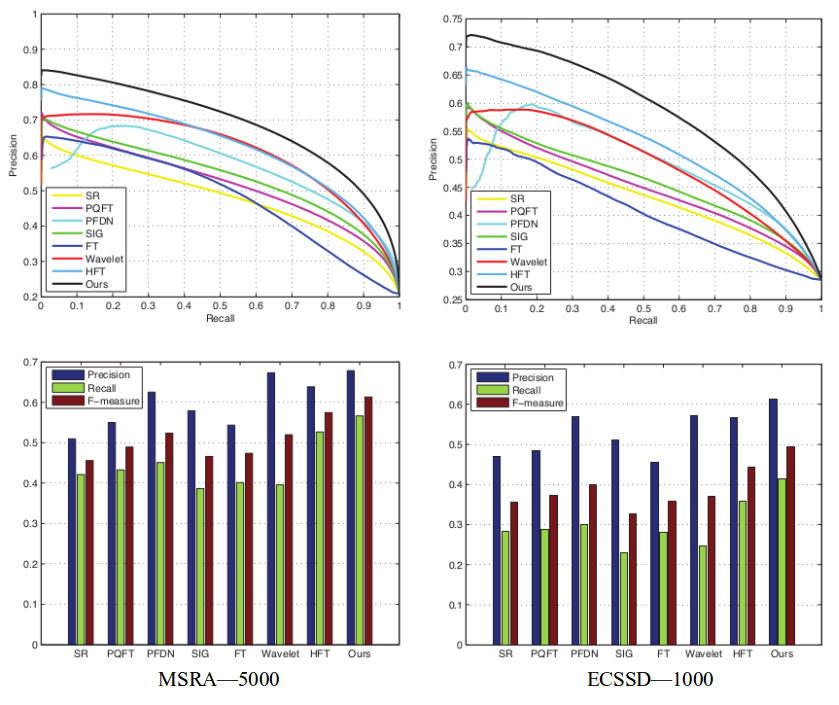
\includegraphics[width=0.48\linewidth]{pr11.png}%
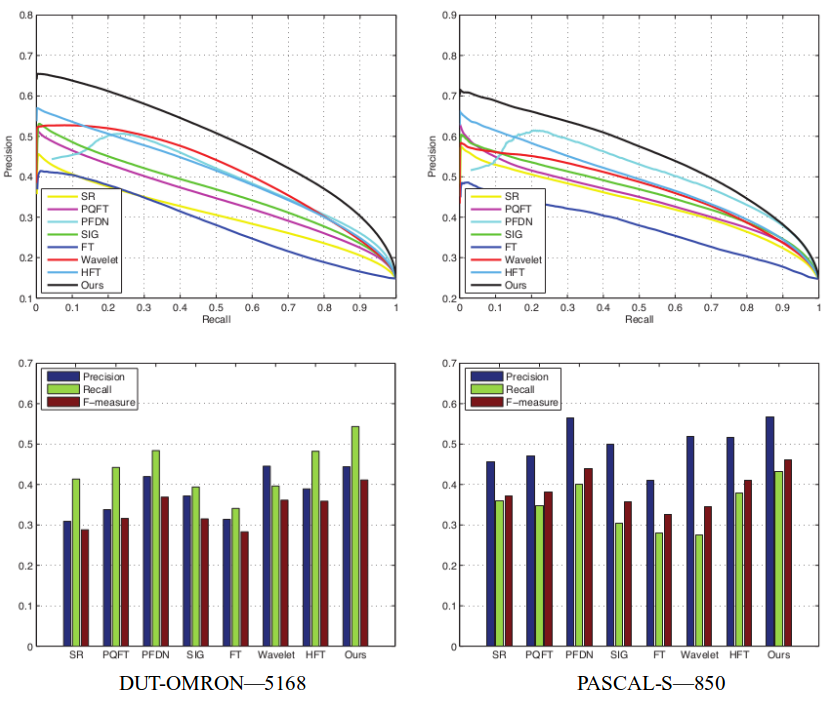
\includegraphics[width=0.48\linewidth]{pr12.png}%
\end{center}
%\centering{\scriptsize \kaishu 精度-召回率曲线和F-测量值。从左到右分别为MSRA数据集和ECSSD数据集; 从上到下分别是不同方法在对应数据集上测得的结果,上面是精度-召回率曲线,下面是F-测量值。}
\end{frame}


%------------------------------------------------------------------------------------------------------------------------------
%\begin{frame}
%  \frametitle{实验结果}
%\begin{center}
%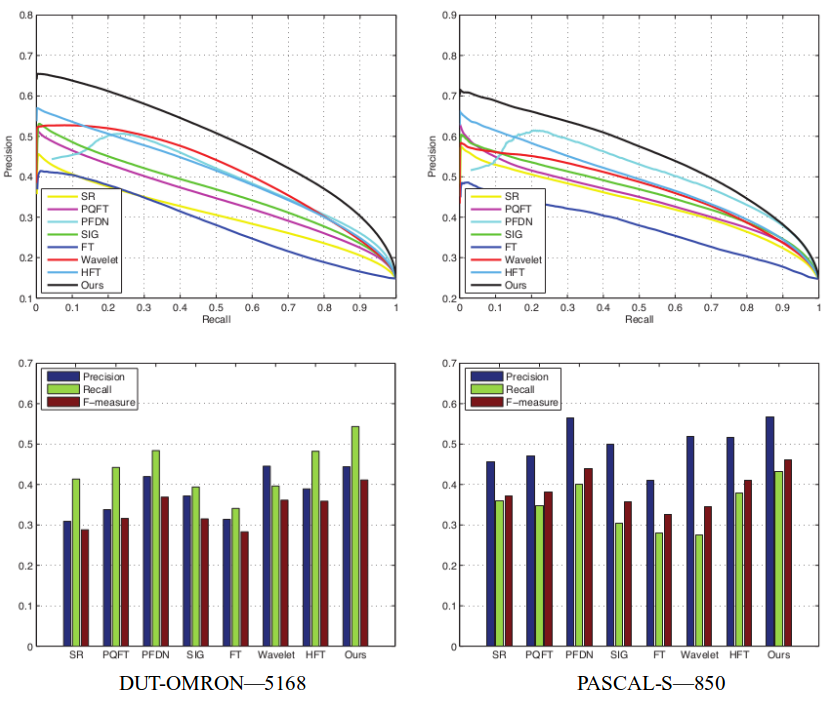
\includegraphics[width=0.6\linewidth]{pr12.png}%
%\end{center}
%\centering{\scriptsize \kaishu 精度-召回率曲线和F-测量值。从左到右分别为DUT-OMRON数据集和PASCAL-S数据集; 从上到下分别是不同方法在对应数据集上测得的结果,上面是精度-召回率曲线,下面是F-测量值。}
%\end{frame}

%------------------------------------------------------------------------------------------------------------------------------
\begin{frame}
  \frametitle{实验结果——显著图}
\begin{center}
\includegraphics[width=0.55\linewidth]{图4_16.jpg}%
\end{center}
%\centering{\scriptsize \kaishu 不同算法在不同数据集上的显著性检测结果}
\end{frame}

%=============================================================================================================================
\section{总结和展望}

%-----------------------------------------------------------------------------------------------------------------------------
\begin{frame}
  \frametitle{总结}
  \begin{enumerate}
  \item 介绍了频域显著性检测的原理和一般处理流程;
  \item 总结了多种典型的频域显著性检测算法;
  \item 提出了基于幅度谱分析的自适应显著目标检测算法。
  \end{enumerate}
\end{frame}

%-----------------------------------------------------------------------------------------------------------------------------
\begin{frame}
  \frametitle{展望}
  \begin{enumerate}
  \item 将频域显著性检测与空间域显著性检测方法结合以提高检测速度和精度;
  \item 进一步研究显著目标尺寸的检测精度;
  \item 引入自顶向下的显著性检测方法。
  \end{enumerate}
\end{frame}

%=============================================================================================================================
\begin{frame}
\vspace{2cm}

\centering{\color{blue} \kaishu \Huge{ \emph{\textbf{  谢谢!}}}}\\
\vspace{1.5cm}

\begin{flushright}
\emph{\href{mailto:zhaohongmiao0627@226.com}{\textrm {Hongmiao~Zhao}}}\\
\href{http://www.ouc.edu.cn}{\textrm {Ocean University of China}}\\
\emph{\textrm {2015.05.23}}
\end{flushright}  
\end{frame}

\end{document}
